\documentclass[12pt]{article}

\usepackage{amsmath}
\usepackage{amssymb}
\usepackage{amsthm}
\usepackage{graphicx}
\usepackage{setspace}
\usepackage{caption}
\usepackage{subcaption}
\usepackage{float}
\usepackage[margin=1in]{geometry}
\usepackage{listings}
\usepackage{textcomp}
\usepackage{multicol}
\usepackage[toc,page]{appendix}
\usepackage{listings}
\usepackage{fancyvrb}
\usepackage{hyperref}
\usepackage{lstbayes}

\usepackage[usenames,dvipsnames]{color}
\definecolor{DGrey}{gray}{0.25}
\definecolor{MGrey}{gray}{0.50}
\definecolor{LGrey}{gray}{0.75}

\usepackage[ruled,vlined,linesnumbered]{algorithm2e}
\newcommand\mycommfont[1]{\footnotesize\ttfamily\textcolor{Gray}{#1}}
\SetCommentSty{mycommfont}

\usepackage{inconsolata}

\usepackage[parfill]{parskip}
\setlength{\parindent}{0pt}
\setlength{\parskip}{\baselineskip}

\newcommand{\et}{e^{i\theta}}
\newcommand{\oo}{\mathcal{O}}
\newcommand{\skipline}{\bigskip\bigskip\bigskip}

\lstdefinestyle{Rsty} { 
    language=R,                         % the language of the code
    basicstyle=\footnotesize\ttfamily,  % the size of the fonts that are used for the code
    numbers=left,                       % where to put the line-numbers
    numberstyle=\footnotesize\color{LGrey},      % the style that is used for the line-numbers
    stepnumber=1,                       % the step between two line-numbers. If it is 1, each line
                                        % will be numbered
    numbersep=5pt,                      % how far the line-numbers are from the code
    backgroundcolor=\color{white},      % choose the background color. You must add \usepackage{color}
    showspaces=false,                   % show spaces adding particular underscores
    showstringspaces=false,             % underline spaces within strings
    showtabs=false,                     % show tabs within strings adding particular underscores
    frame=single,                       % adds a frame around the code
    rulecolor=\color{black},            % if not set, the frame-color may be changed on line-breaks within not-black text (e.g. commens (green here))
    tabsize=2,                          % sets default tabsize to 2 spaces
    captionpos=b,                       % sets the caption-position to bottom
    breaklines=true,                    % sets automatic line breaking
    breakatwhitespace=false,            % sets if automatic breaks should only happen at whitespace
    keywordstyle=\color{DGrey},     % keyword style
    commentstyle=\color{LGrey},   % comment style
    stringstyle=\color{MGrey},    % string literal style
    literate={<-}{{$\gets$}}1,           % prettier assignment arrows
    xleftmargin=4.0ex,
    deletekeywords={I,density,rect,_,palette,data,scale,panel,R,frame,labels,options}
}

\lstnewenvironment{R}
{\lstset{style=Rsty}}
{}

\lstdefinestyle{Cppsty} { 
    language=C++,                         % the language of the code
    basicstyle=\footnotesize\ttfamily,  % the size of the fonts that are used for the code
    numbers=left,                       % where to put the line-numbers
    numberstyle=\footnotesize\color{LGrey},      % the style that is used for the line-numbers
    stepnumber=1,                       % the step between two line-numbers. If it is 1, each line
                                        % will be numbered
    numbersep=5pt,                      % how far the line-numbers are from the code
    backgroundcolor=\color{white},      % choose the background color. You must add \usepackage{color}
    showspaces=false,                   % show spaces adding particular underscores
    showstringspaces=false,             % underline spaces within strings
    showtabs=false,                     % show tabs within strings adding particular underscores
    frame=single,                       % adds a frame around the code
    rulecolor=\color{black},            % if not set, the frame-color may be changed on line-breaks within not-black text (e.g. commens (green here))
    tabsize=4,                          % sets default tabsize to 2 spaces
    captionpos=b,                       % sets the caption-position to bottom
    breaklines=true,                    % sets automatic line breaking
    breakatwhitespace=false,            % sets if automatic breaks should only happen at whitespace
    keywordstyle=\color{DGrey},     % keyword style
    commentstyle=\color{LGrey},   % comment style
    stringstyle=\color{MGrey},    % string literal style
    %literate={<-}{{$\gets$}}1,           % prettier assignment arrows
    xleftmargin=4.0ex,
    deletekeywords={T}
}

\lstnewenvironment{CPP}
{\lstset{style=Cppsty}}
{}

\lstdefinestyle{Stansty} { 
    language=Stan,                         % the language of the code
    basicstyle=\footnotesize\ttfamily,  % the size of the fonts that are used for the code
    numbers=left,                       % where to put the line-numbers
    numberstyle=\footnotesize\color{LGrey},      % the style that is used for the line-numbers
    stepnumber=1,                       % the step between two line-numbers. If it is 1, each line
                                        % will be numbered
    numbersep=5pt,                      % how far the line-numbers are from the code
    backgroundcolor=\color{white},      % choose the background color. You must add \usepackage{color}
    showspaces=false,                   % show spaces adding particular underscores
    showstringspaces=false,             % underline spaces within strings
    showtabs=false,                     % show tabs within strings adding particular underscores
    frame=single,                       % adds a frame around the code
    rulecolor=\color{black},            % if not set, the frame-color may be changed on line-breaks within not-black text (e.g. commens (green here))
    tabsize=2,                          % sets default tabsize to 2 spaces
    captionpos=b,                       % sets the caption-position to bottom
    breaklines=true,                    % sets automatic line breaking
    breakatwhitespace=false,            % sets if automatic breaks should only happen at whitespace
    keywordstyle=\color{DGrey},     % keyword style
    commentstyle=\color{LGrey},   % comment style
    stringstyle=\color{MGrey},    % string literal style
    %literate={<-}{{$\gets$}}1,           % prettier assignment arrows
    xleftmargin=4.0ex,
    deletekeywords={T}
}

\lstnewenvironment{Stan}
{\lstset{style=Stansty}}
{}

\renewcommand{\arraystretch}{2}

\begin{document}

\noindent
{\LARGE {\bf Spatial Epidemics} }
\\\\
Dexter Barrows\\
\today

\section{Spatial SIR}

	Spatial epidemic models provide a way to capture not just the temporal trend in an epidemic, but to also integrate spatial data and infer how the infection is spreading in both space and time. One such model we can use is a dynamic spatiotemporal SIR model.

	We wish to construct a model build upon the stochastic SIR compartment model described previously but one that consists of several connected spatial locations, each with its own set of compartments. Consider a set of locations numbered $i = 1, ..., N$, where $N$ is the number of locations. Further, let $N_i$ be the number of neighbours location $i$ has. The model is then

	\begin{equation}
		\begin{aligned}
			\frac{dS_i}{dt} & = - \left( 1 - \phi \frac{N_i}{N_i + 1} \right) \beta_i S_i I_i - \left( \frac{\phi}{N_i + 1} \right) S_i \sum_{j = 0}^{N_i} \beta_j I_j \\
			\frac{dI_i}{dt} & = \left( 1 - \phi \frac{N_i}{N_i + 1} \right) \beta_i S_i I_i + \left( \frac{\phi}{N_i + 1} \right) S_i \sum_{j = 0}^{N_i} \beta_j I_j - \gamma I \\
			\frac{dR_i}{dt} & = \gamma I,
		\end{aligned}
	\end{equation}
    
	Neighbours for a particular location are numbered $j = 1, ..., N_i$. We have a new parameter, $\phi \in [0,1]$, which is the degree of connectivity. If we let $\phi = 0$ we have total spatial isolation, and the dynamics reduce to the basic SIR model. If we let $\phi = 1$ then each of the neighbouring locations will have weight equivalent to the parent location.

	As before we let $\beta$ embark on a geometric random walk defined as

	\begin{equation}
		\beta_{i, t+1} = \exp \left( \log(\beta_{i, t}) + \eta (\log(\bar{\beta}) - \log(\beta_{i, t})) + \epsilon_{t} \right).
	\end{equation}
	
	Note that as $\beta$ is a state variable, each location has its own stochastic process driving the evolution of its $\beta$ state.

	If we imagine a circular topology in which each of $10$ locations is connected to exactly two neighbours (i.e. location $1$ is connected to locations $N$ and $2$, location $2$ is connected to locations $1$ and $3$, etc.), and we start each location with completely susceptible populations except for a handful of infected individuals in one of the locations, we obtain a plot of the outbreak progression in Figure [\ref{dataplot}].

	\begin{figure}[H]
        \centering
        \captionsetup{width=.8\linewidth}
        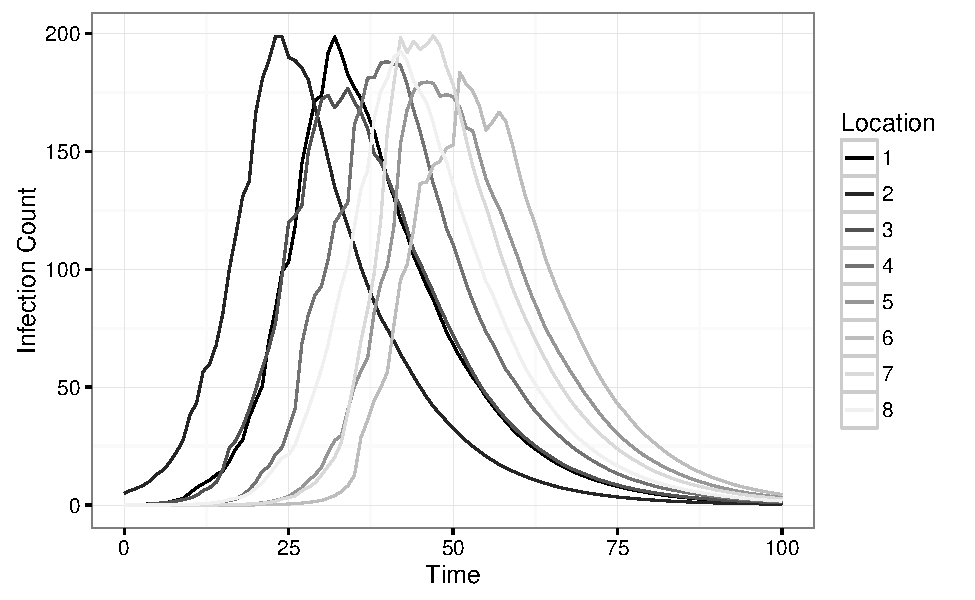
\includegraphics[width=0.8\textwidth]{./images/dataplot.pdf}
        \caption{Evolution of a spatial epidemic in a ring topology. The outbreak was started with 5 cases in Location 2. Parameters were $R_0 = 3.0$, $\gamma = 0.1$, $\eta = 0.5$, $\sigma_{err} = 0.5$, and $\phi = 0.5$.}
        \label{dataplot}
    \end{figure}

    If we add noise to the data from Figure [\ref{dataplot}], we obtain Figure [\ref{dataplot2}], below.

    \begin{figure}[H]
        \centering
        \captionsetup{width=.8\linewidth}
        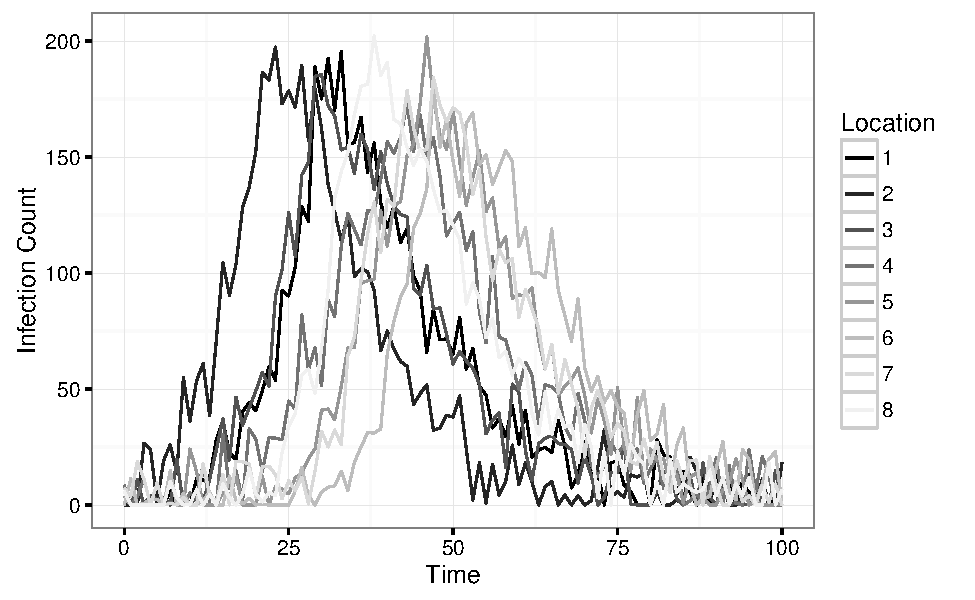
\includegraphics[width=0.8\textwidth]{./images/dataplot2.pdf}
        \caption{Evolution of a spatial epidemic as in Figure [\ref{dataplot}], with added observation noise drawn from $\mathcal{N}(0,10)$.}
        \label{dataplot2}
    \end{figure}


\section{Dewdrop Regression}



\newpage
\begin{appendices}

	\section{Spatial SIRS R Function Code}

		R code to simulate the outlined Spatial SIR function.

		\lstinputlisting[style=Rsty]{../../code/sir-functions/StocSSIR.r}

	\section{RStan Spatial SIR Code}

	    This code implements a Spatial SIR model in Rstan.

	    \lstinputlisting[style=Rsty]{../../code/hmc/hmc-spa/sir-spa-euler.stan}

    \section{IF2 Spatial SIR Code}

	    This code implements a Spatial SIR model using IF2 in C++.

	    \lstinputlisting[style=Cppsty]{../../code/if2/if2-spa/if2-spa.cpp}

\end{appendices}



\end{document}